\chapter{Efficient optimization of sparsity and smoothness regularized models}\label{chap:efficient_opt}
\markright{{~{\rm \ref{chap:efficient_opt}}. Efficient optimization of sparsity and smoothness regularized models}\hfill}{}

\minitoc

\newthought{Though the SpaceNet models} introduced in equations \eqref{eq:opt_pb} of chapter \ref{chap:structured_priors} lead to superior estimators compared to classical estimators (Ridge regression, SVM, etc.) without spatial penalization, they are considerably harder to optimize than these classical models. Indeed, the corresponding optimization problems is non-separable in the model coefficients, and except for the case of GraphNet~\citep{hebiri2011,grosenick2013} and social-sparsity~\citep{kowalski2013social,varoquaux2016social},
the penalty term $\mathcal P(\w)$ is neither smooth nor proximable\footnote{
A function $f$ is said to be \textit{proximable} if its operator $\text{prox}_{\gamma f}$ is easy to compute. This is the case for $\ell_p$-norms  (with $ p \ge 1$, to ensure convexity) and indicator functions of simple closed convex sets like balls, simplexes, half-spaces, etc.}.
For the penalty to fully exercise its
structuring effect on the maps, this optimization problem must be
solved to a good tolerance resulting in a computational challenge. Lack of good solver and explicit control of
tolerance can lead to brain maps and conclusions that reflect
properties of the solver more than of model coefficients, as illustrated in Fig. \ref{Fig:benchmarks_prni}.

  %% \begin{itemize}
  %% \item{proximal methods}
  %%   \begin{itemize}
  %%     \item single-step\\
  %%       {-} ISTA (Iterative Soft-Thresholding Algorithm)   \citep{daubechies2004}
  %%     \item multi-step / accelerated\\
  %%       {-} FISTA (Fast ISTA)   \citep{beck09fista}
  %%   \end{itemize}
  %% \item {primal-dual \& splitting methods}
  %%   \begin{itemize}
  %%   \item ADMM (Alternating Directions Method of Multipliers)   \citep{boyd2011distributed}
  %%     % (\textit{Alternating Directions Method of Multipliers})
  %%   \item Chambolle-Pock's Primal-Dual   \citep{chambolle2010}
  %%   \end{itemize}
  %% \item {quasi-Newton methods}
  %%   \begin{itemize}
  %%   \item HANSO ({Hybrid Algorithm for Non-smooth Optimization})   \citep{lewis2008}
  %%   \item L-BFGS   \citep{ciyou1994} on smooth surrogates of the penalty
  %%   \end{itemize}
  %% \end{itemize}
  

%% \begin{figure*}
%%   \begin{subfigure}[t]{1\linewidth}
%%     \hspace*{-.01\linewidth}%
%%     \includegraphics[width=.6\linewidth]{haxby_lr_energy.pdf}
%%     \hspace*{-.09\linewidth}%
%%     \includegraphics[width=.6\linewidth]{haxby_lr.pdf}%
%%     % \vspace{-2ex}
%%     \caption{\textbf{Classification} with logistic regression model
%%       \eqref{eq:opt_pb}. on the visual recognition face-house
%%     discrimination task. \textbf{Left}: excess energy $E(\mathbf{w}_t) -
%%     E(\mathbf{w})_{t \rightarrow \infty}$ as a function 
%%     of time.
%%     \textbf{Right}: convergence time of the various solvers for different
%%     choice of regularization parameters.
%%     Broken lines correspond to a tolerance of $10^{0}$,
%%     whilst full-lines correspond to $10^{-2}$.  The thick vertical line
%%     indicates the best model selected by cross-validation.}
%%     \label{Fig:HaxbyLR}
%%   \end{subfigure}
%%   \begin{subfigure}[t]{1\linewidth}
%%     \includegraphics[width=.6\linewidth]{haxby_mse.pdf}%
%%     \hspace{-.09\linewidth}%
%%     % generate with: ipython ../wip/tv_l1_solver/plot_parallel_plots.py poldrack_mse_12th.json 2e1 --pdb
%%     \includegraphics[width=.6\linewidth]{poldrack_mse.pdf}
%%     % \vspace{-2ex}
%%     \caption{\textbf{Regression.} results. \textbf{Left}:
%%       on the visual recognition  face-house discrimination task; \textbf{Right}: on the
%%       Mixed gambles dataset. Broken lines correspond to a tolerance of $10^{0}$,
%%       whilst full-lines correspond to $10^{-2}$. The thick vertical line
%%       indicates the best model selected by cross-validation.}
%%     \label{Fig:MSEtimes}
%%   \end{subfigure}
%% \caption{Benchmarks for different solvers for the TV-$\ell_1$ model
%%   \eqref{eq:opt_pb} on the visual recognition face-house
%%   discrimination task. See   \citep{dohmatob2014benchmarking} for more details.}
%% \end{figure*}

\section{Solving TV-L1 regularized problems}
The optimization problem \eqref{eq:opt_pb} is very challenging:
it is non-smooth (except in the case of Laplacian regularization), non-separable and heavily ill-conditioned. For the penalty to fully exercise its
structuring effect on the maps, this optimization problem must be
solved to a good tolerance resulting in a computational challenge.
In \citep{dohmatob2014benchmarking}, we did an extensive study of all solvers applicable to the problem in TV-$\ell_1$ special case (which happens to be the most difficult scenario).
Our results outlined the best strategy: a double FISTA loop, where the
inner loop computes the proximal operator of the penalty term, with approximate precision on the duality-gap. This was further refined and implemented in  \citep{varoquaux2015faasta}.
\begin{figure}[!htb]
  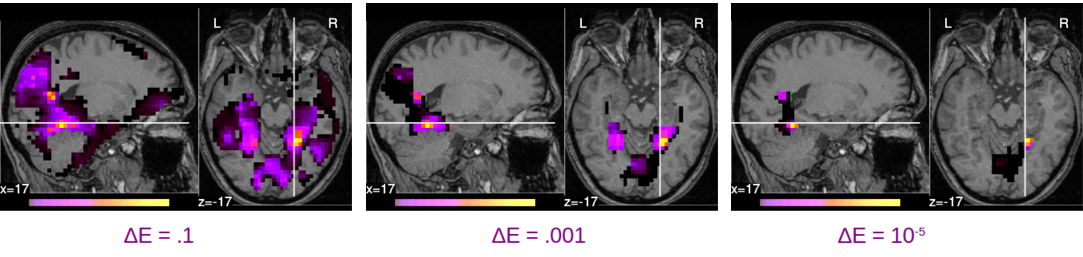
\includegraphics[width=1.\linewidth]{tvl1_why_optimize.png}%
\caption{TV-$\ell_1$ maps for the face-house discrimination task on
  the visual recognition dataset.
  Note that
  the stopping criterion is defined as a threshold on the energy
  decrease per one iteration of the algorithm, and thus differs from
  the tolerance displayed in figure \ref{Fig:benchmarks_prni}.  This figure shows
  the importance of convergence for problem \eqref{eq:opt_pb}, and motivates
  the need for fast solvers for SpaceNet priors, especially the non-smooth ones like TV-$\ell_1$ and Sparse Variation. See~\citep{dohmatob2014benchmarking} for details.}
  \label{Fig:benchmarks_prni}
\end{figure}

% In  \citep{dohmatob2014benchmarking}, we explored a wide variety of solvers and exhibited their
% convergence properties on fMRI data. Below we present a brief overview of the paper.

\subsection{The algorithms}
\paragraph{ISTA/FISTA.}
ISTA~ \citep{daubechies2004}, and its accelerated variant
FISTA~ \citep{beck2009a}, are proximal gradient approaches: the go-to
methods for non-smooth optimization. In their seminal introduction of TV
for fMRI,  \citep{michel2011} relied on ISTA.
The challenge of these methods for TV is that the proximal operator
%% \footnote{The proximal operator (or prox for short) can be seen as a generalization of projection unto convex set.}
  of TV
cannot be computed exactly; we approximate it in an inner FISTA loop
 \citep{beck2009b,michel2011}.
% ,  \citep{gramfort-etal:2013a}.
%%  and must itself be solved by a
%% FISTA\footnote{Note that solving TV and TV$-\ell_1$ are formally very
%% close  \citep{gramfort-etal:2013a}.
% }
%  \citep{beck2009b,michel2011}. 
Here, for all FISTA implementations we use
the faster monotonous FISTA variant  \citep{beck2009b}. We control the
optimality of the TV proximal via its dual gap  \citep{michel2011} and
use a line-search strategy in the monotonous FISTA to decrease the
tolerance as the algorithm progresses, ensuring convergence of the
TV-$\ell_1$ regression with good accuracy. See~\citep{dohmatob2014benchmarking,varoquaux2015faasta}.

\paragraph{ISTA/FISTA with backtracking.}
A key ingredient in FISTA's convergence is the Lipschitz
constant $L_{\nabla \ell}$, of the derivative of smooth part of the objective function
. The tighter the upper bound used for this constant,
the faster the resulting FISTA algorithm. In FISTA, the main use of 
$L_{\nabla \ell}$ is the fact that: for any
stepsize $0 < t \le 1/L_{\nabla \ell}$ and for any point $\mathbf{z}$,
% \begin{shaded}
\begin{equation}%
  \begin{gathered}
    \ell(\mathbf{p}_{t}(\mathbf{z})) \le
    \ell(\mathbf{z}) + \mathbf{r}_{t}^T\nabla
    \ell(\mathbf{z}) + \frac{1}{2t} \|\mathbf{r}_{t}\|_{2}^2,
    \text{  where} \quad\\
    \mathbf{p}_{t}(\mathbf{z}) := \textrm{prox}_{\alpha t \mathcal P}(\mathbf{z} - t
    \nabla \ell(\mathbf{z})) \,\text{  and  }\,
    \mathbf{r}_{t} :=
    \mathbf{p}_{t}(\mathbf{z}) - \mathbf{z} \quad
  \end{gathered}
  \label{eq:fista_ineq}
\end{equation}
% \end{shaded}
In least-squares regression, $L_{\nabla \ell}$ is precisely the largest
singular value of the design matrix $\mathbf{X}$.
For logistic
regression however, the tightest known upper bound for
$L_{\nabla \ell}$ is $\|\mathbf{X}\|\|\mathbf{X}^T\|$,
% (for example see Appendix A of ~\citep{yuan2012}),
which performs very poorly locally (i.e, stepsizes $\sim 1 / L_{\nabla \ell}$ are
sub-optimal locally). A way to circumvent this difficulty is
\emph{backtracking line search} ~\citep{beck2009a}, where one tunes the
stepsize $t$ to satisfy inequality \eqref{eq:fista_ineq} locally at
point $\mathbf{z}$. 


\paragraph{ADMM: Alternating Direction Method of Multipliers.}
ADMM is a Bregman Operator Splitting primal-dual method for
solving convex-optimization problems by splitting the
objective function in two convex terms which are functions of linearly-related auxiliary variables
~\citep{boyd2010}.  ADMM is particularly appealing for problems such as TV
regression: using the variable split $\mathbf{z}
\leftarrow \nabla \mathbf{w}$, the regularization is a simple $\ell_{1}/\ell_2$
norm on $\mathbf{z}$ for which the proximal is exact and computationally
cheap. However, in our settings, limitations of ADMM are:
\begin{itemize}
\item The $\mathbf{w}$-update involves the inversion of a large $p$-by-$p$
  ill-conditioned linear operator (precisely a weighted sum of
  $\mathbf{X}^T\mathbf{X}$, the laplacian $\Delta$, and the identity
  operator).
\item The dual stepsize parameter $\nu$ in the penalization of the split
  residual $\frac{1}{2}\nu\|\mathbf{z} - \nabla \mathbf{w}\|_2^2$ is hard to set (this is still an
  open problem), and though under mild conditions ADMM
  converges for any value of $\nu$, the convergence rate depends
  on $\nu$. In chapter \ref{chap:admm}, we study the rate of convergence of ADMM on the kinds
  of penalized
  least squares regression problem considered in this manuscript, and derive some theoretical
  results.
\end{itemize}

\paragraph{Primal-Dual algorithm of Chambolle and Pock ~\citep{chambolle2010}.}
This scheme is another method based on operator splitting.
Used for fMRI TV regression by ~\citep{gramfort-etal:2013a},
it does not require setting a hyperparameter.  % XXX : this is wrong you have the tau / sigma
However it is a first-order single-step method and is thus more impacted by the
conditioning of the problem. Note that here we explore this primal-dual
method only in the squared loss setting, in which the algorithm can be accelerated by
precomputing the SVD of $\mathbf{X}$ ~\citep{gramfort-etal:2013a}
.

\paragraph{HANSO ~\citep{lewis2008}.}
a modified LBFGS scheme based on gradient 
sampling methods ~\citep{burke2005} and inexact
line-search. For non-smooth problems as in our case, the algorithm relies on
random initialization, to avoid singularities with high probability. 
Here, we used the original authors' implementation.

\paragraph{Uniform approximation by smooth convex surrogates.}
The $\ell_{1}$ norm (resp. TV semi-norm) is differentiable everywhere with
gradient $\left(w_j/|w_j|\right)_{j \in [\![p]\!]}$ (resp. $-\dive (((\nabla \mathbf{w})_j/\|(\nabla \mathbf{w})_j\|_2)_{j \in [\![p]\!]}))$), except when some voxels are inactive with
$w_j = 0$ (resp. $(\nabla \w)_j = 0$), corresponding to black spots (resp. edges).  A convenient
approach (see for example ~\citep{NESTA, nesterov2005a, nesterov2005b,
  beck2012}) for dealing with such singularities is to uniformly
approximate the offending function with smooth surrogates that
preserve its convexity. Given  % I removed "and other important properties"
a smoothing parameter $\mu > 0$, we define \emph{smoothed} versions
of $\ell_1$ and TV:
%
\begin{eqnarray}
    \|\mathbf{w}\|_{1,\mu} := \sum_j
    \sqrt{\mathbf{w}_j^2 + \mu^2},\;
    \|\mathbf{w}\|_{\text{TV}, \mu} :=
    \sum_{j} \sqrt{\|(\nabla \mathbf{w})_j\|_{2}^2 + \mu^2}
\end{eqnarray}
These surrogate upper-bounds are convex and everywhere-differentiable
with gradients that are Lipschitz-continuous with constants $1/\mu$ and
$\|\nabla\|^2(1/\mu) = 12 / \mu$ respectively.
They lead to smoothed versions of problem \eqref{eq:opt_pb}:
\begin{align}
  \mathbf{\hat{w}}_{\mu} := \argmin_{\mathbf{w}}\;
  \{E_{\mu}(\mathbf{w}) := \ell(\mathbf{w}) + \alpha
    \mathcal P_{\text{TV-L1},\mu}(\mathbf{w})\},
  \label{eq:sopt_pb}
\end{align}
where    $\mathcal P_{\text{TV-L1},\mu}(\mathbf{w}) :=\rho \|\mathbf{w}\|_{1,\mu} +
(1 - \rho)\|\mathbf{w}\|_{\text{TV}, \mu}$.

To solve \eqref{eq:opt_pb}, we consider problems of the form
\eqref{eq:sopt_pb} with $\mu \rightarrow 0^+$: we start with a coarse
$\mu$ ($= 10^{-2}$, \emph{e.g}) and cheaply solve the $\mu$-smoothed problem
\eqref{eq:sopt_pb} to a precision $\sim \mu$ using a fast
iterative oracle like the LBFGS~\citep{ciyou1994}; we
obtain a better estimate for the solution; then we decrease $\mu$ by a fixed factor,
and restart the solver on problem \eqref{eq:sopt_pb} with this solution; and so on, in a 
\emph{continuation} process~\citep{NESTA} detailed in Alg.
\ref{Tab:pseudocode_lbfgs}.
This algorithm is not faster than
$\mathcal{O}(1/\epsilon)$: indeed a first-order algorithm
for the sub-problem \eqref{eq:sopt_pb} has optimal worst-case iteration complexity $\mathcal{O}(\sqrt{L_{\mu}/\epsilon})$
~\citep{nesterov1983}, and $L_{\mu} \sim 1 / \mu \sim 1 / \epsilon$. We
believe that this bound is tight but a detailed analysis is
beyond the scope of this manuscript.
\begin{algorithm}
  \caption{LBFGS algorithm with continuation}
  \label{Tab:pseudocode_lbfgs}  
  \begin{algorithmic}[1]  
    \Require $\epsilon > 0$ the desired precision, $\beta$ ($0 < \beta <
    1$) the rate of decay of the smoothing parameter $\mu$, and $\gamma > 0$ be a constant.
    Finally,
    let LBFGS: $(E_\mu, \mathbf{w}^{(0)}, \epsilon) \mapsto \mathbf{w}$ be
    an oracle which when warm-started with an initial guess
    $\mathbf{w}^{(0)}$, returns an $\epsilon$-optimal
    solution (i.e $E_\mu(\mathbf{w}) - E_\mu^{*} < \epsilon$) for problem \eqref{eq:sopt_pb}.\\
    \textbf{Initialize} $ 0 < \mu^{(0)}$ ($= 10^{-2}$, \emph{e.g}),
    $\mathbf{w}^{(0)}\in \mathbb{R}^p$, and $k = 0$.
    \While{$\gamma\mu^{(k)} \ge \epsilon$}
    \State $\mathbf{w}^{(k + 1)} \leftarrow \mbox{LBFGS}(E_{\mu^{(k)}}, \mathbf{w}^{(k)}, \gamma\mu^{(k)})$
    \State $\mu^{(k + 1)} \leftarrow \beta \mu^{(k)}$
    \State $k \leftarrow k + 1$
    \EndWhile
  \end{algorithmic}
\end{algorithm}

\subsection{Experiments on fMRI datasets}
\label{sec:experiments}
We now detail experiments done on publicly available
data. All experiments were run full-brain without spatial smoothing.

\paragraph{Visual recognition.}
\label{subsec:haxby}
Our first benchmark dataset is a popular block-design fMRI dataset from a study on face and
object representation in human ventral temporal cortex ~\citep{haxby2001}.
It consists of
6 subjects with 12 runs per subject. In each run, the subjects
passively viewed images of eight object categories, grouped
in 24-second blocks separated by intermittent rest periods. This
experiment is a classification task: predicting the object category. We use a
two-class prediction target: $\mathbf{y}$ encodes faces versus houses.
The design matrix $\mathbf{X}$ is made of
time-series from the full-brain mask of $p = 23\,707$ voxels over $n =
216$ TRs, of a single subject (subj1).

\paragraph{Mixed Gambles.}
Our second benchmark dataset is a study in which
subjects were presented with mixed (gain/loss) gambles, and decided
whether they would accept each gamble~\citep{mixedgambles2007}.  No outcomes of these gambles
were presented during scanning, but after the scan three gambles were
elected at random and played for real money. The prediction task here is
to predict the magnitude of the gain and thus a regression on a
continuous variable~\citep{jimura2012}. The data
The are pulled from 16 subjects with 48 3D scans each, making up for a total of $n=768$ samples with approximately $p=3.3 \times 10^4$ voxels.

% We validate our algorithms on both simulated and real data.
\smallskip

We study the convergence of the algorithms for parameters close to the
optimal parameters set by 10-fold cross-validation to maximize prediction
accuracy.

\subsection{Results: convergence times}
 \begin{pagefigure}%[!htbp]
   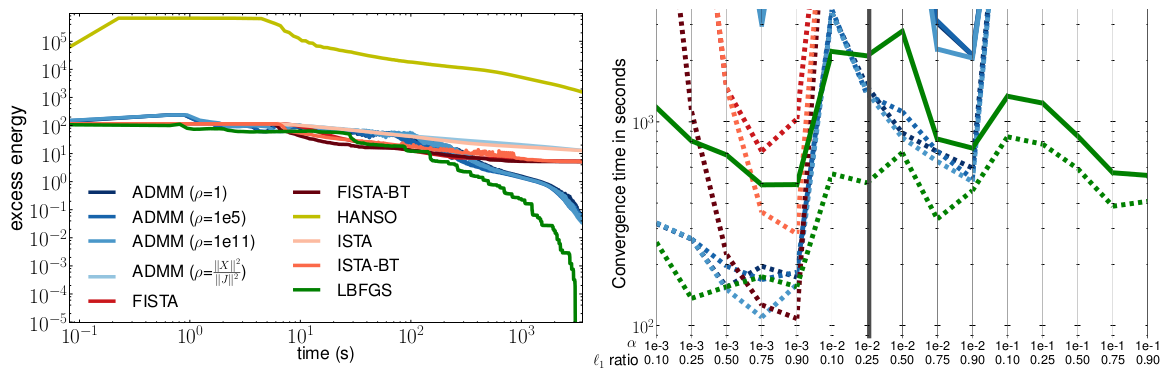
\includegraphics[width=1\linewidth]{figures/solvers_1.png}
   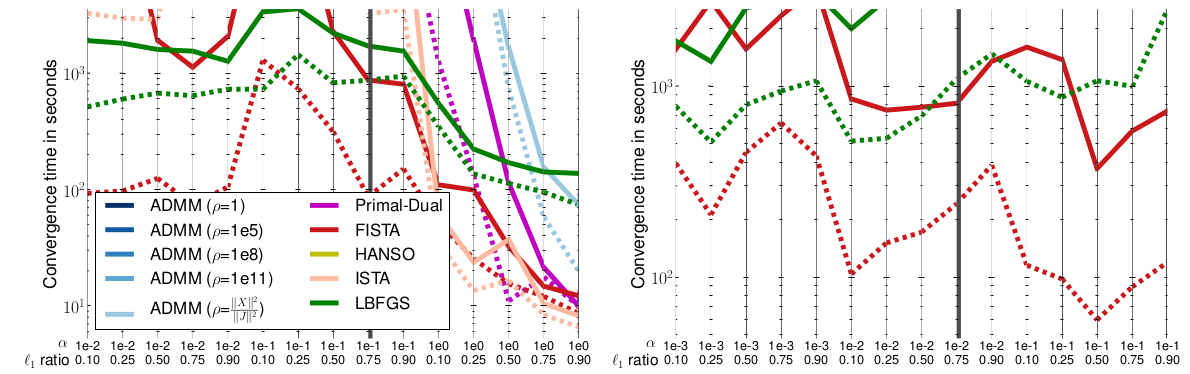
\includegraphics[width=1\linewidth]{figures/solvers_2.png}
   \caption{\textbf{Benchmarking } solvers for TV-$\ell_1$ penalized models. \textbf{Top:} TV-$\ell_1$ penalized Logistic Regression on the visual recognition face-house discrimination task. \textbf{Top Left:} excess energy $E(\B{w}_t ) - E(\B{w}^*)$ as a function of time. \textbf{Top Right:} convergence time of the various solvers for different choice of regularization parameters. Broken lines correspond to a tolerance of
     $10^0$ , whilst full-lines correspond to $10^{-2}$ . The thick vertical line indicates the best model selected by cross-validation. \textbf{Bottom:} TV-$\ell_1$ penalized Least-Squares Regression. \textbf{Bottom Left:} on the visual recognition face-house discrimination task; \textbf{Bottom Right:} on the Mixed gambles dataset. The thick vertical line indicates the best model selected by cross-validation.}
   \label{fig:tvl1bench}
\end{pagefigure}

\label{sec:results}
Here, we present benchmark results for our experiments. Figure
\ref{fig:tvl1bench} gives results for the logistic regression run on the
visual recognition dataset: convergence plots of energy as a function of
time show that all methods are asymptotically decreasing. The left part of
Fig. \ref{fig:tvl1bench}
shows the time required to give a convergence
threshold, defined as a given excess energy compared to the lowest energy
achieved by all methods, for different choices of regularization
parameters. Similarly, the right part of Fig. \ref{fig:tvl1bench} shows convergence times
for squared loss on both datasets. For these figures,
each solver was run for a maximum of 1 hour per problem. Solvers that do
not appear on a plot did not converge for the corresponding
tolerance and time budget.

For logistic loss, the most serious contender is
algorithm \ref{Tab:pseudocode_lbfgs}, LBFGS applied on a smooth
surrogate, followed by ADMM, however ADMM performance
varies markedly depending on the choice of $\rho$ (more on this in chapter \ref{chap:admm}). For the squared loss
FISTA and algorithm \ref{Tab:pseudocode_lbfgs} are the best performers,
with FISTA achieving a clear lead for the larger mixed-gambles dataset.
Note that in the case of strong regularization the problem is better
conditioned, and first-order methods such as the
primal-dual approach can perform well.

\bibliographystyle{plainnat}
\bibliography{bib_all}
